\chapter{Comunicazione su canali Rumorosi}
Abbiamo parlato già all'inizio del capitolo di un esempio di canale rumoroso e di alcuni semplici tecniche di rilevamento e correzione degli errori. Essendo i \textbf{canali reali rumorosi}, il nostro obiettivo è esaminare se è possibile usare un canale rumoroso per comunicare in modo \textbf{affidabile}.

\section{Canali Rumorosi}
\paragraph{Definizione di Canale discreto memoryless}
Un \textbf{canale discreto memoryless} $Q$ è caratterizzato da un alfabeto di \textbf{input} $A_X$, un alfabeto di \textbf{output} $A_Y$ e un insieme di distribuzioni di probabilità $Pr[y|x]$, ognuna per ogni $x\in A_X$.\\
Queste probabilità di transizione possono essere memorizzate in una matrice:
\begin{equation}
	Q_{j|i} = Pr[y = b_j | x = a_i] \qquad 
	\begin{cases}
		\text{j-esima riga} \\
		\text{i-esima colonna}
	\end{cases}
\end{equation}

\subsubsection{Definizione di capacità di canale}
La capacità di un canale $Q$ definisce la massima mutua informazione:
\begin{equation}
	C(Q) = \max_{P_X}\ I(X;Y)
\end{equation}

La distribuzione $P_X$ per cui ottieniamo il massimo di $I(X;Y)$ è chiamata \textbf{distribuzione input ottimale}.


\subsection{Esempi di canali rumorosi}
\textbf{Canale Binario Simmetrico}:

Dati $A_X = \{0,1\}$  e $A_Y = \{0,1\}$ abbiamo:\\
\begin{minipage}{0.25\textwidth}
	\begin{figure}[H]
		\centering
		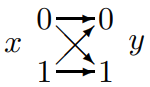
\includegraphics[width=0.7\textwidth]{images/cbs.png}
	\end{figure}
\end{minipage}
\begin{minipage}{0.50\textwidth}
	$$
	P(y = 0|x= 0) = 1 -f;\quad P(y = 0| x=1) = f;
	$$
	$$
	P(y=1|x=0) = f;\quad P(y=1|x=1) = 1 - f;
	$$
\end{minipage}
\begin{minipage}{0.25\textwidth}
	\begin{figure}[H]
		\centering
		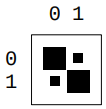
\includegraphics[width=0.5\textwidth]{images/prCbs.png}
	\end{figure}
\end{minipage}

\textbf{Z-Channel}:

Dati $A_X = \{0,1\}$  e $A_Y = \{0,1\}$ abbiamo:\\
\begin{minipage}{0.25\textwidth}
	\begin{figure}[H]
		\centering
		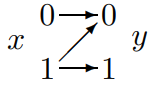
\includegraphics[width=0.7\textwidth]{images/zchan.png}
	\end{figure}
\end{minipage}
\begin{minipage}{0.50\textwidth}
	$$
	P(y = 0|x= 0) = 1;\quad P(y = 0| x=1) = f;
	$$
	$$
	P(y=1|x=0) = 0;\quad P(y=1|x=1) = 1 - f;
	$$
\end{minipage}
\begin{minipage}{0.25\textwidth}
	\begin{figure}[H]
		\centering
		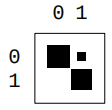
\includegraphics[width=0.5\textwidth]{images/prZchan.png}
	\end{figure}
\end{minipage}

\textbf{Noisy Typewriter}:

Dati $A_X = A_Y = \{\verb|A|, \verb|B|, \verb|C|, \cdots, \verb|Z|, \verb|-|\}$. Le 27 lettere sono raggruppate in un cerchio e quando il dattilografo (typist) prova a scrivere (ad esempio) \verb|B|, il risultato può essere \verb|A,B| o \verb|C|, con ognuno probabilità $\frac{1}{3}$.\\
La lettera finale '\verb|-|' simboleggia la lettera \verb|A|\\
\begin{minipage}{0.20\textwidth}
	\begin{figure}[H]
		\centering
		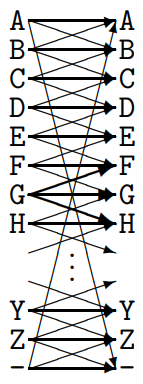
\includegraphics[width=0.6\textwidth]{images/ntype.png}
	\end{figure}
\end{minipage}
\begin{minipage}{0.50\textwidth}
	$$
	Pr(y = A|x= B) = \frac{1}{3}
	$$
	$$
	Pr(y = B|x= B) = \frac{1}{3}
	$$
	$$
	Pr(y = C|x= B) = \frac{1}{3}
	$$
\end{minipage}
\begin{minipage}{0.25\textwidth}
	\begin{figure}[H]
		\centering
		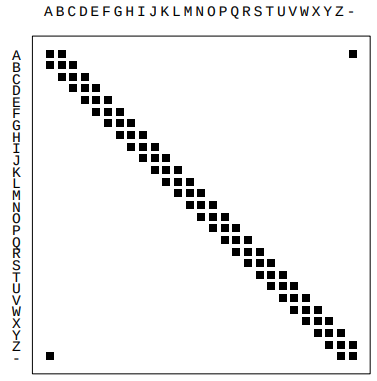
\includegraphics[width=1.2\textwidth]{images/prNtype.png}
	\end{figure}
\end{minipage}

\newpage
\textbf{Esempio N.1 - Mutua Informazione su Canale Binario Simmetrico}

Supponiamo che $f=0.15$ e che $P_X = \{p_0 = 0.9\ , p_1 = 0.1\}$. Calcoliamo $I(X;Y)$

Innanzitutto calcoliamo $Pr[y=0]$ e $Pr[y=1]$.
$$
Pr[y=0] = Pr[y=0|x=0]\cdot Pr[x=0] + Pr[y=0|x=1]\cdot Pr[x=1] = (1-f)\cdot p_0 + f\cdot p_1 = 
$$
$$
0.85 \cdot 0.9 + 0.15 \cdot 0.1 = 0.78
$$
$$
Pr[y=1] = Pr[y=1|x=0]\cdot Pr[x=0] + Pr[y=1|x=1]\cdot Pr[x=1] = f\cdot (1- p_0) + (1-f)\cdot p_1 = 
$$
$$
0.15 \cdot 0.9 + 0.85 \cdot 0.1 = 0.22
$$

Per calcolare $I(X;Y) = H(Y) - H(Y|X)$, devo prima calcolare $H(Y)$ e $H(Y|X)$. Cominciamo con $H(Y)$:
$$
H(Y) = - Pr[y=0] \log_2 Pr[y=0] + Pr[y=1] \log_{2} Pr[y=1] =
$$
$$
= \left(0.78 \cdot \log_2 (0.78) + 0.22 \cdot \log_2 (0.22) \right) = H(Pr[y=1]) = H(0.22) = 0.76
$$

Prima di calcolare $H(Y|X)$ dobbiamo ricavare $H(Y|x=0)$ e $H(Y|x=1)$. Cominciamo con $H(Y|x=0)$:
$$
H(Y|x=0) = Pr[y=0|x=0] \log_2 (Pr[y=0|x=0]) + Pr[y=1|x=0] \log_2 (Pr[y=1|x=0]) =
$$
$$
= (1-f)\log_2 (1-f) + f \log_2 f = H(f)
$$

Adesso calcoliamo $H(Y|x=1)$:
$$
H(Y|x=1) = Pr[y=0|x=1] \log_2 (Pr[y=0|x=1]) + Pr[y=1|x=1] \log_2 (Pr[y=1|x=1]) =
$$
$$
= f \log_2 f + (1-f)\log_2 (1-f) = H(f)
$$

Infine calcoliamo $H(Y|X)$:
$$
-\sum_{x\in X}\sum_{y\in Y} Pr[X=x,\ Y=y]\ \log_2 (Pr[Y=y|X=x]) = \sum_{x\in X} Pr[X=x] H(Y|X=x) = 
$$
$$
= p_0\ H(Y|x=0) + p_1 H(Y|x=1) = 0.9\ H(f) + 0.1\ H(f) = H(f) = H(0.15) = 0.61
$$

Calcoliamo la Mutua Informazione:
$$
I(X;Y) = H(0.22) - H(0.15) = 0.76 - 0.61 = 0.15\ \text{bit}
$$

\textbf{Possiamo fare meglio di così? Si, infatti calcolando la capacità di canale}:
$$
C(Q_{BSC}) = H(0.5) - H(0.15) = 1.0 - 0.61 = 0.39\ \text{bit}
$$

\begin{figure}[h]
	\centering
	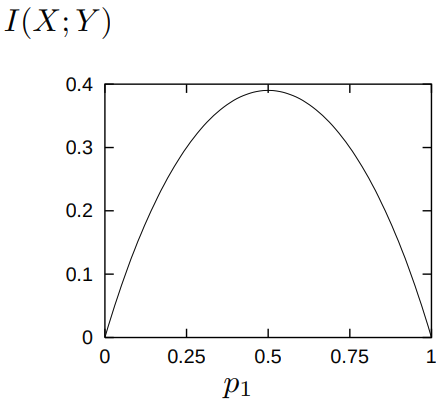
\includegraphics[width=0.5\textwidth]{images/QCBS}
\end{figure}

\newpage

\textbf{Esempio N.2 - Mutua Informazione su Z-Channel}

Supponiamo che $f=0.15$ e che $P_X = \{p_0 = 0.9\ , p_1 = 0.1\}$. Dobbiamo ricavare $I(X;Y)$
$$
H(Y) = H(Pr[y=1]) = H((1-f)\cdot p_1) = 0.42
$$
$$
Pr[y=0] = Pr[y=0|x=0]\cdot Pr[x=0] + Pr[y=0|x=1]\cdot Pr[x=1] =
$$
$$
0 + (1-f)\cdot p_1 = 0.85\cdot 0.1 = 0.085
$$
Calcoliamo $H(Y|X)$:
$$
H(Y|X) = H(Y|x=0)\ Pr[x=0] + H(Y|x=1)\ Pr[x=1] =
$$
$$
H(Pr[y=1|x=0])\ p_0 + H(Pr[y=1|x=1])\ p_1 = 0 + H(1-f)p_1 = H(0.85) \cdot 0.1 = 0.61 \cdot 0.1 = 0.061
$$
Adesso calcoliamo $I(X;Y)$
$$
I(X;Y) = H((1-f)\cdot p_1) - p_1\cdot H(1-f) = 0.42 - 0.061 = 0.36\ \text{bit}
$$

Questa funzione in $p_1^* = 0.445$ con $f=0.15$ non è banale.
La capacità di canale $C(Q_Z) = 0.685\ \text{bit}$

\begin{figure}[h]
	\centering
	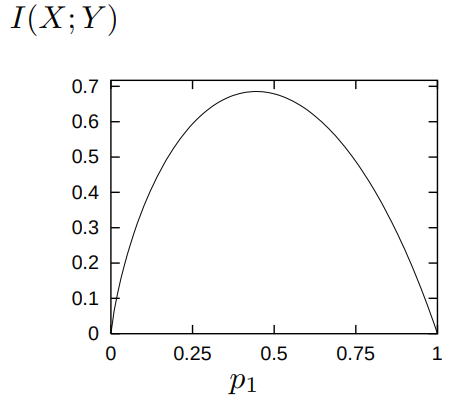
\includegraphics[width=0.5\textwidth]{images/QZchan}
\end{figure}

\textbf{Esempio N.3 - Capacità del Noisy Typewriter Channel}

Si trova che la distribuzione ottimale input è la distribuzione uniforme che dà:
$$
C(Q_{NT}) = \log_{2} 9 = 3,17\ \text{bit}
$$

\subsection{Teorema del Codice di un Canale Rumoroso}
La capacità di canale misura la frequenza di quanti \textbf{blocchi di informazione} possono essere trasferiti nel canale con una \textit{piccola quantità di errore arbitraria}.

\subsubsection{$(N,K)$ codici a blocco}
Un $(N,K)$ codice a blocco per un canale $Q$ è una lista di $S=2^K$ codeword tali che:
\begin{equation}
	{x^{(1)}, x^{(2)}, \cdots, x^{(2^K)}}, \quad x^{(s)}\in A_X^N
\end{equation}
ognuna con lunghezza $N$. Ci permette di codificare $S = 2^K$ segnali usando blocchi di lunghezza $N$.

\textit{OSSERVAZIONE}: Il numero di codewords $S$ è un intero, ma il numero di bit necessario per scegliere una codeword, ovvero $K\equiv \log_2 S$, non è necessariamente un intero.

\newpage
\subsubsection{Tasso di comunicazione}
Il tasso di comunicazione del codice per canale è:
\begin{equation}
	R = \frac{K}{N}\ \text{bit}
\end{equation}

\textit{OSSERVAZIONE}: Questa definizione è usata per qualsiasi canale, tuttavia se il canale non ha un alfabeto di input binario e contiene $q$ simboli, il tasso di comunicazione diventa:
\begin{equation}
	R = \frac{K}{N \log_{2} q}\ \text{bit} 
\end{equation}

\subsubsection{Decoder per $(N,k)$ codici a blocco}
Un decoder per $(N,k)$ codici a blocco mappa da un insieme di stringhe di output $S$ di lunghezza $N$, ovvero $A_Y^N$, un segnale $$\hat{s} \in \{0,1,2,\cdots,2^K\}$$

\textit{OSSERVAZIONE}: Il simbolo $\hat{s} = 0$ può essere usato per indicare un \textbf{fallimento}.

\subsubsection{Probabilità di un errore di blocco}
La \textbf{probabilità di un errore di blocco} di un codice e di un decoder, dato un canale e una distribuzione di probabilità sul segnale codificato $P(s_{in})$ è:
\begin{equation}
	p_B = \sum_{s_{in}} P(s_{in})\cdot P(s_{out} \neq s_{in}|s_{in})
\end{equation}

\subsubsection{Probabilità massima di un errore di blocco}
La probabilità \textbf{massima} di un errore di blocco è:
\begin{equation}
	p_{BM} = \max_{s_{in}} P(s_{out} \neq s_{in}|s_{in})
\end{equation}

\subsubsection{Probabilità di errore di bit}
Assumendo che $s$ sia rappresentato da un da un vettore binario \textbf{s} di lunghezza $K$, la probabilità di bit error consiste nella probabilità media che che un bit dell’output sia
diverso dal corrispondente bit dell’input.
\begin{equation}
	p_b = \max_{s} \left(\frac{1}{k} \sum_{i=1}^{k} Pr[\hat{s}(i) \neq s(i)|s]\right)
\end{equation}

\subsubsection{Decoder Ottimale}
Il decoder ottimale per un dato canale è quello che minimizza la probabilità di \textbf{errore di blocco}.\\ 
Decodifica un output $y$ come $\hat{s}$ che ha la massima probabilità a posteriori:
\begin{equation}
	p[s|y] = \frac{[y|s]\cdot p[s]}{\sum_{s'_{\text{input}}} P(y|s')\cdot P(s')}
\end{equation}

con: $\hat{s_{\text{output}}} = \text{argmax}\ P(s|y)$
\newpage
\subsection{Teorema di Shannon per canali rumorosi}
Il Teorema di compone di tre parti:
\begin{enumerate}
	\item Per ogni canale discreto di tipo \textbf{memoryless}, la capacità di canale:
	\begin{equation}
		C = \max_{P_X} I(X;Y)
	\end{equation}
	ha la seguente proprietà. Per ogni $\varepsilon > 0$, $R < C$ ed $N$ sufficientemente grande, esiste un codice di lunghezza $N$ e tasso $\geq R$ ed un decoder tale che la probabilità di block error massima è $< \varepsilon$.
	
	\item Se si ammette una probabilità di bit error $p_b$, tassi fino a
	\begin{equation}
		R(p_b) = \frac{C}{1 - H_2(p_b)}
	\end{equation}
	\textbf{sono possibili}.
	
	\item Per ogni $p_b$ tassi maggiori di $R(p_b)$ \textbf{non sono possibili}.
\end{enumerate}

\subsubsection{Conferma del Teorema di Shannon per canali rumorosi sul Noisy Typewriter Channel}

Possiamo creare una strategia di comunicazione completamente \textbf{priva di errori} usando un codice a blocchi di lunghezza $N=1$.\\ Usiamo come alfabeto un sottoinsieme di $A_X$ formato dalle lettere ogni 3: \verb|B,E,H,|$\cdots$\verb|,Z| 

Ognuno di questi simboli può essere \textbf{univocamente decodificato} scegliendo la decodifica come il simbolo più vicino di $A_X$. Questo sottoinsieme d'input ha 9 elementi e il tasso di comunicazione è uguale alla capacità del canale NT:
$$
Q(C_{NT}) = \log_2 9
$$

\begin{figure}[h]
	\centering
	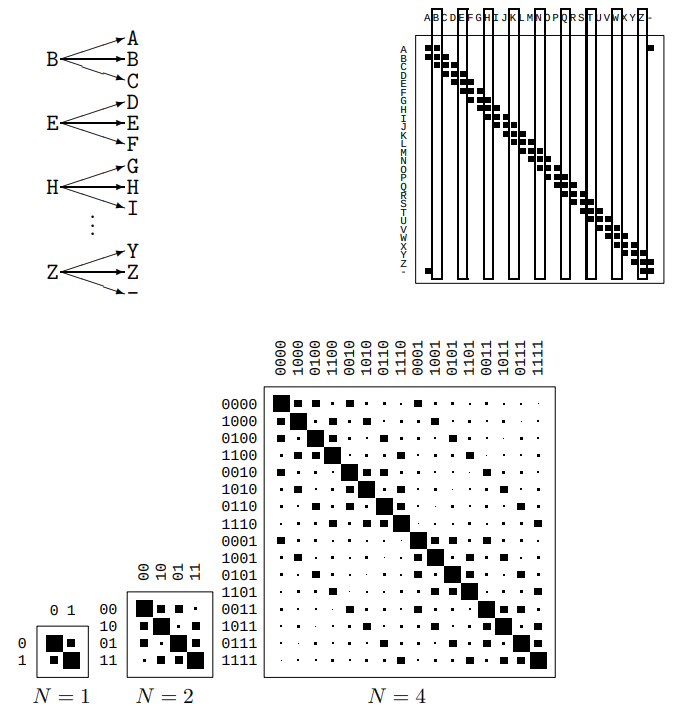
\includegraphics[width=0.8\textwidth]{images/proofNT.png}
\end{figure}


